\setcounter{ExampleCounter}{1}
\begin{center}
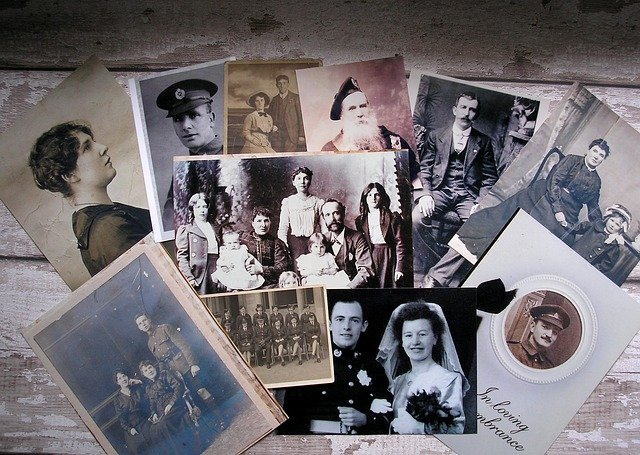
\includegraphics[width=0.8\textwidth]{genealogy}
\end{center}
If you've ever studied your genealogy, one of the most basic ways to visualize it is by using a \emph{family tree}, like the one shown below for a portion of the British royal family.  In this tree, each node represents a member of the royal family by birth.  If that member has children, the other parent of those children is shown in red.
\begin{center}
\begin{tikzpicture}
  \GraphInit[vstyle=simple]
  \tikzset{VertexStyle/.append style={scale=0.3}}
  
  \Vertex[x=0,y=0]{Elizabeth}
  \Vertex[x=-4.5,y=-2]{Charles}
  \Vertex[x=-2,y=-2]{Anne}
  \Vertex[x=2,y=-2]{Andrew}
  \Vertex[x=4.5,y=-2]{Edward}
  
  \Vertex[x=-6,y=-4]{William}
  \Vertex[x=-3,y=-4]{Harry}
  
  \Vertex[x=0.5,y=-4]{Beatrice}
  \Vertex[x=3.5,y=-4]{Eugenie}
  
  \Vertex[x=-6,y=-6]{George}
  \Vertex[x=-4,y=-6]{Charlotte}
  \Vertex[x=-2,y=-6]{Louis}
  
  \tikzset{VertexStyle/.append style={scale=0.05}}
  \Vertex[x=0,y=-2]{level1}
  \Vertex[x=-4.5,y=-4]{level2a}
  \Vertex[x=2,y=-4]{level2b}
  \Vertex[x=-6,y=-4.5]{level3a}
  \Vertex[x=-4,y=-4.5]{level3b}
  \Vertex[x=-4,y=-5.5]{level4b}
  \Vertex[x=-6,y=-5.5]{level4a}
  \Vertex[x=-2,y=-5.5]{level4c}
  
  \extralabel{Elizabeth}{90}{\parbox{1in}{\centering Elizabeth II, Queen of England\\ {\color{red}Philip, Duke of Edinburgh}}}
  \extralabel{Charles}{90}{\parbox{1in}{\centering Charles, Prince of Wales\\ {\color{red}Diana Spencer}}}
  \extralabel{Anne}{90}{\parbox{1in}{\centering Anne, Princess Royal}}
  \extralabel{Andrew}{90}{\parbox{1in}{\centering Andrew, Duke of York\\ {\color{red}Sarah Ferguson}}}
  \extralabel{Edward}{90}{\parbox{0.75in}{\centering Edward, Earl of Wessex}}
  
  \extralabel{William}{90}{\parbox{1in}{\centering William, Duke of Cambridge\\ {\color{red}Catherine Middleton}}}
  \extralabel{Harry}{90}{\parbox{1in}{\centering Harry, Duke of Sussex}}
  
  \extralabel{Beatrice}{-90}{\parbox{1in}{\centering Beatrice}}
  \extralabel{Eugenie}{-90}{\parbox{1in}{\centering Eugenie}}
  
  \extralabel{George}{-90}{\parbox{1in}{\centering George}}
  \extralabel{Charlotte}{-90}{\parbox{1in}{\centering Charlotte}}
  \extralabel{Louis}{-90}{\parbox{1in}{\centering Louis}}
  
  \Edge(Elizabeth)(level1)
  \Edge(Charles)(Edward)
  \Edge(Charles)(level2a)
  \Edge(William)(Harry)
  \Edge(Andrew)(level2b)
  \Edge(Beatrice)(Eugenie)
  \Edge(William)(level3a)
  \Edge(level3a)(level3b)
  \Edge(level3b)(level4b)
  \Edge(level4a)(level4c)
  \Edge(level4a)(George)
  \Edge(level4b)(Charlotte)
  \Edge(level4c)(Louis)
\end{tikzpicture}
\end{center}

The\marginnote{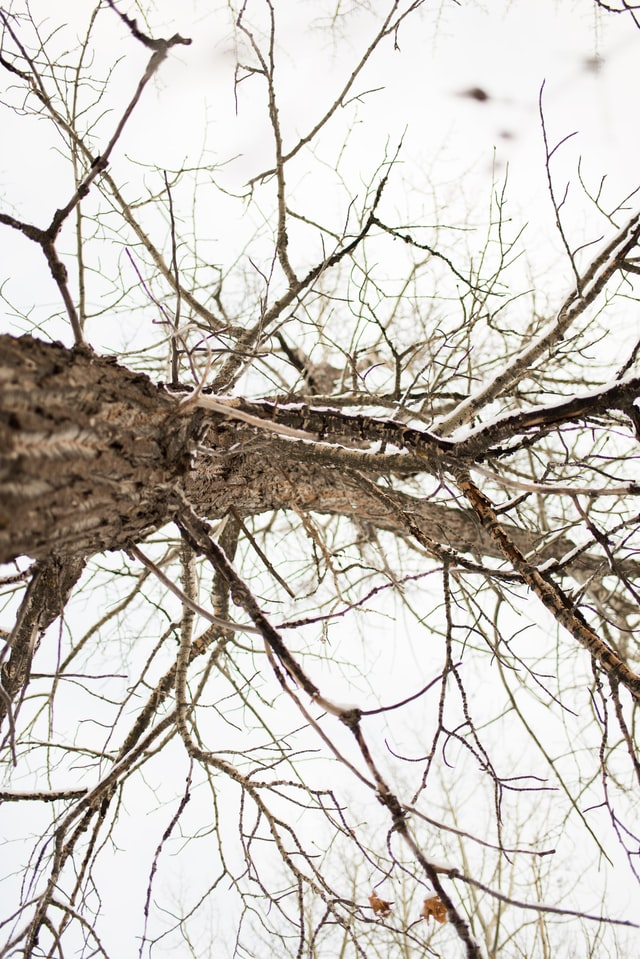
\includegraphics[width=1in]{tree_branch}} terminology of a tree and branches is clear, because the family tree above has the same structure as a physical tree, with branches that lead to smaller branches, and so on.\\

In graph theory, we borrow this term of a \emph{tree} for a graph that has this same structure.  Now, it can be hard to identify the defining feature of a tree branch, but notice that the main pattern is that none of the branches loop back to reconnect with the rest of the tree; once you head down a particular edge, there's no way to get back where you were without returning along that edge.  This leads us to the definition of a tree (watch out; the definition is so terse that it can be hard to grasp at first).

\begin{formula}{Trees}
A \textbf{tree} is a connected graph with no simple circuits.
\end{formula}

Let's make sure that makes sense: a tree is a graph where a path down a particular branch won't find itself looping back and reconnecting; that path is only connected to the rest of the graph at one point.  Therefore, there can't be any simple circuits, because to return to a point that we left earlier, we'd have to retrace our steps.\\

Now, it turns out that there are a few equivalent ways to identify a tree.  Each of the following is an equivalent definition for a tree: a graph $G$ is a tree if
\begin{itemize}
\item There is a unique simple path between any two nodes (not particularly helpful for identification).
\item $G$ is connected, but barely; removing any edge would make it disconnected (think about cutting a branch from a tree--that branch doesn't hang there, connected at a another point).  This can be easy to check visually: see if you can find any edges that you can remove and still leave the graph connected.
\item $G$ is connected, and there are $n-1$ edges, where $n$ is the number of nodes (this one is easy to check too, since it just involves counting).
\end{itemize}

\begin{example}[https://www.youtube.com/watch?v=NNRIIWfwauE&list=PLfmpjsIzhztst_PxJXo574wshSwxU9Yg_&index=10]{Identifying Trees}
Which of the following are trees?
\begin{center}
\begin{tabular}{c c c}
\begin{tikzpicture}
  \GraphInit[vstyle=simple]
  \tikzset{VertexStyle/.append style={scale=0.3}}
  \SetGraphUnit{1.4}
  
  \Vertex{a}
  \EA(a){b}
  \SO(a){c}
  \SOEA(a){d}
  \SO(c){e}
  \EA(e){f}

  \extralabel{a}{90}{$a$}
  \extralabel{b}{90}{$b$}
  \extralabel{c}{180}{$c$}
  \extralabel{d}{0}{$d$}
  \extralabel{e}{-90}{$e$}
  \extralabel{f}{-90}{$f$}
  
  \Edge(a)(c)
  \Edge(b)(c)
  \Edge(d)(c)
  \Edge(f)(c)
  \Edge(e)(f)
\end{tikzpicture}
\hspace*{0.2in}
&
\hspace*{0.2in}
\begin{tikzpicture}
  \GraphInit[vstyle=simple]
  \tikzset{VertexStyle/.append style={scale=0.3}}
  \SetGraphUnit{1.4}
  
  \Vertex{a}
  \EA(a){b}
  \SO(a){c}
  \SOEA(a){d}
  \SO(c){e}
  \EA(e){f}

  \extralabel{a}{90}{$a$}
  \extralabel{b}{90}{$b$}
  \extralabel{c}{180}{$c$}
  \extralabel{d}{0}{$d$}
  \extralabel{e}{-90}{$e$}
  \extralabel{f}{-90}{$f$}
  
  \Edge(a)(c)
  \Edge(a)(b)
  \Edge(a)(d)
  \Edge(b)(e)
  \Edge(c)(f)
  \Edge(d)(e)
\end{tikzpicture}
\hspace*{0.2in}
&
\hspace*{0.2in}
\begin{tikzpicture}
  \GraphInit[vstyle=simple]
  \tikzset{VertexStyle/.append style={scale=0.3}}
  \SetGraphUnit{1.4}
  
  \Vertex{a}
  \EA(a){b}
  \SO(a){c}
  \SOEA(a){d}
  \SO(c){e}
  \EA(e){f}
  \SO(e){g}
  \EA(g){h}

  \extralabel{a}{90}{$a$}
  \extralabel{b}{90}{$b$}
  \extralabel{c}{180}{$c$}
  \extralabel{d}{0}{$d$}
  \extralabel{e}{180}{$e$}
  \extralabel{f}{0}{$f$}
  \extralabel{g}{-90}{$g$}
  \extralabel{h}{-90}{$h$}
  
  \Edge(a)(d)
  \Edge(b)(d)
  \Edge(d)(c)
  \Edge(e)(g)
  \Edge(g)(h)
  \Edge(h)(f)
\end{tikzpicture}\\
& & \\
(a)
\hspace*{0.2in}
&
\hspace*{0.2in}
(b)
\hspace*{0.2in}
&
\hspace*{0.2in}
(c)
\end{tabular}
\end{center}

\sol
\begin{enumerate}[(a)]
\item This is a tree, because it \emph{is} connected, but removing any edge would create disconnected components.  We could also count the nodes and edges, and note that there is one fewer edge than the number of nodes.
\item This is not a tree.  Again, we could count the nodes and edges, or try removing edges to see if any leave it connected, but we can also note that there are simple circuits, like $a \to d \to e \to b \to a$ in this graph.
\item This is not a tree, because it is not connected.  However, since each of the components are trees themselves, this could be called a \textbf{forest}.
\end{enumerate}

Our conclusion is that \boxtext{(a) is the only tree}\ .
\end{example}

There\marginnote{\emph{for instance, trees can be used to describe games; chess programs do this, as one example}} are many, many applications of trees, but we will only discuss two of them: \textbf{binary search trees} and \textbf{spanning trees}.
\pagebreak

\subsection{Binary Search Trees}
Searching through a list is a hard problem.  If you were handed a randomly sorted list of names and told to find a particular one, you'd have to simply read through every name, and you could expect on average to have to read half of the list before finding the name.  Think of how often you use a search function in your life, and it becomes obvious that we need searching to be as efficient as possible.\\

One way to make searching more efficient is to sort the items.  Say, for example, the list of names you were given was ordered alphabetically; would that make your job easier?  Of course it would.  Say, for instance, you were looking for the name Kayla: you would know to look near the middle of the list, and if your eye fell on the M's, you'd know to go backward.  Similarly, if you started at the G's, you'd know to go forward.\\

This is the basic concept of a \emph{binary search tree}; the word \emph{binary} simply refers to two possibilities.  In the alphabetically ordered list, you have two options: go forward or go backward, so in that case, you're really doing a binary search.\\

It turns out that there is an efficient way to use a tree to encode an ordered list like this, and there are advantages to this that have to do with the way that computers can read the tree.  Below is an example of a tree that can be used to search for names in the following list: Leah, Callista, Priya, Lucy, Jason, Sergio, Sonia, Dennis, and Adrian.

\begin{center}
\begin{tikzpicture}[scale=0.75]
  \GraphInit[vstyle=simple]
  \tikzset{VertexStyle/.append style={scale=0.3}}
  
  \Vertex[x=0,y=0]{Leah}
  \Vertex[x=-4,y=-2]{Callista}
  \Vertex[x=4,y=-2]{Priya}
  \Vertex[x=-6,y=-4]{Adrian}
  \Vertex[x=-2,y=-4]{Jason}
  \Vertex[x=2,y=-4]{Lucy}
  \Vertex[x=6,y=-4]{Sergio}
  \Vertex[x=-4,y=-6]{Dennis}
  \Vertex[x=8,y=-6]{Sonia}
  
  \extralabel{Leah}{90}{Leah}
  \extralabel{Callista}{135}{Callista}
  \extralabel{Priya}{45}{Priya}
  \extralabel{Adrian}{135}{Adrian}
  \extralabel{Jason}{60}{Jason}
  \extralabel{Lucy}{120}{Lucy}
  \extralabel{Sergio}{45}{Sergio}
  \extralabel{Dennis}{135}{Dennis}
  \extralabel{Sonia}{45}{Sonia}
  
  \Edge(Leah)(Callista)
  \Edge(Leah)(Priya)
  \Edge(Callista)(Adrian)
  \Edge(Callista)(Jason)
  \Edge(Priya)(Lucy)
  \Edge(Priya)(Sergio)
  \Edge(Jason)(Dennis)
  \Edge(Sergio)(Sonia)
\end{tikzpicture}
\end{center}

Notice the structure of this tree: first of all,\marginnote{\textbf{Binary Tree:} each node has one \emph{parent} and at most two children} it is called a \textbf{binary tree} because at each level, a node will have at most two branches coming out of it and going down to the next level (we can say that each node will have at most two \emph{children}, if we view this like a family tree).\\

Next, the reason this tree can be used for searching is that it is \textbf{sorted}: notice that at each node, if you turn to the left and follow a branching path, all the names along that path will be \emph{before} the original one, and if you go to the right, all the names will come \emph{after} it, alphabetically.  For instance, if you start with Priya, on the left-hand branch you'll find Lucy (before Priya alphabetically), and on the right-hand branch, you'll find Sergio and Sonia (both after Priya alphabetically).  This is what makes it a binary \emph{search} tree.\\

Say you are searching for the name Jason.  Start at the top of the tree, and compare Jason to the name there: Leah.  Since Jason comes before Leah alphabetically, we know Jason will be in the left branch, so head to the left.  Now, pause here, and notice that we've immediately eliminated about half of the possible names in the list from consideration; we don't have to search through those.  This is the major feature of binary search trees, since by eliminating about half of the remainder of the list at every step, we can hone in on our search term very quickly.\\

Back to the search: we're heading down the left branch, looking for Jason.  The next name we encounter is Callista, and since Jason comes after that alphabetically, we take a turn to the right, which brings us to our result.  Notice that this only took two steps, and we found the right name out of a list of 9.  The efficiency of this method only gets more dramatic as the list gets bigger.
\pagebreak

\begin{example}[https://www.youtube.com/watch?v=A31V6w6qtus&list=PLfmpjsIzhztst_PxJXo574wshSwxU9Yg_&index=11]{Building a Binary Search Tree}
Build a binary search tree for the following list of words, starting with the first word at the top of the tree:
\begin{center}
\emph{location, solution, promotion, decision, city, bread,\\ enthusiasm, writer, signature, criticism}
\end{center}

\sol
Start with the word \emph{location} at the top.  To add the word \emph{solution}, note that it comes after \emph{location} alphabetically, so create a node to the right.
\begin{center}
\begin{tikzpicture}[scale=0.6]
  \GraphInit[vstyle=simple]
  \tikzset{VertexStyle/.append style={scale=0.3}}
  
  \Vertex[x=0,y=0]{location}
  \Vertex[x=4,y=-2]{solution}
  
  \extralabel{location}{90}{location}
  \extralabel{solution}{45}{solution}
  
  \Edge(location)(solution)
\end{tikzpicture}
\end{center}

For the next word, \emph{promotion}, start again by comparing it to the top word, \emph{location}.  Since it comes after that, go to the right, and compare it to the word there, \emph{solution}.  This time, it comes before the comparison word, so we turn to the left, and since there's nothing there, we drop \emph{promotion} in that spot.
\begin{center}
\begin{tikzpicture}[scale=0.6]
  \GraphInit[vstyle=simple]
  \tikzset{VertexStyle/.append style={scale=0.3}}
  
  \Vertex[x=0,y=0]{location}
  \Vertex[x=4,y=-2]{solution}
  \Vertex[x=2,y=-4]{promotion}
  
  \extralabel{location}{90}{location}
  \extralabel{solution}{45}{solution}
  \extralabel{promotion}{250}{promotion}
  
  \Edge(location)(solution)
  \Edge(solution)(promotion)
\end{tikzpicture}
\end{center}

If we continue this process, we'll eventually get the tree shown below (try it yourself and see if you can get the same tree).

\begin{center}
\begin{tikzpicture}[scale=0.7]
  \GraphInit[vstyle=simple]
  \tikzset{VertexStyle/.append style={scale=0.3}}
  
  \Vertex[x=0,y=0]{location}
  \Vertex[x=-4,y=-2]{decision}
  \Vertex[x=4,y=-2]{solution}
  \Vertex[x=-6,y=-4]{city}
  \Vertex[x=-2,y=-4]{enthusiasm}
  \Vertex[x=2,y=-4]{promotion}
  \Vertex[x=6,y=-4]{writer}
  \Vertex[x=-4,y=-6]{criticism}
  \Vertex[x=4,y=-6]{signature}
  \Vertex[x=-8,y=-6]{bread}
  
  \extralabel{location}{90}{location}
  \extralabel{decision}{135}{decision}
  \extralabel{solution}{45}{solution}
  \extralabel{city}{135}{city}
  \extralabel{enthusiasm}{80}{enthusiasm}
  \extralabel{promotion}{250}{promotion}
  \extralabel{writer}{45}{writer}
  \extralabel{criticism}{0}{criticism}
  \extralabel{signature}{0}{signature}
  \extralabel{bread}{180}{bread}
  
  \Edge(location)(decision)
  \Edge(location)(solution)
  \Edge(decision)(city)
  \Edge(decision)(enthusiasm)
  \Edge(solution)(promotion)
  \Edge(solution)(writer)
  \Edge(promotion)(signature)
  \Edge(city)(bread)
  \Edge(city)(criticism)
\end{tikzpicture}
\end{center}
\end{example}

\begin{try}
Build a binary search tree for the following list of words, starting with the first word:
\begin{center}
\emph{foster, dry, inspire, feign, courage,\\ persist, reactor, inn, advisor, divorce}
\end{center}
\end{try}
\pagebreak

\begin{example}[https://www.youtube.com/watch?v=O_zBszBFcTQ&list=PLfmpjsIzhztst_PxJXo574wshSwxU9Yg_&index=12]{Searching with a Binary Search Tree}
Using the binary tree created in the last example, shown below, search for the word \emph{criticism}.  How many steps (comparisons) are needed to find it?
\begin{center}
\begin{tikzpicture}[scale=0.6]
  \GraphInit[vstyle=simple]
  \tikzset{VertexStyle/.append style={scale=0.3}}
  
  \Vertex[x=0,y=0]{location}
  \Vertex[x=-4,y=-2]{decision}
  \Vertex[x=4,y=-2]{solution}
  \Vertex[x=-6,y=-4]{city}
  \Vertex[x=-2,y=-4]{enthusiasm}
  \Vertex[x=2,y=-4]{promotion}
  \Vertex[x=6,y=-4]{writer}
  \Vertex[x=-4,y=-6]{criticism}
  \Vertex[x=4,y=-6]{signature}
  \Vertex[x=-8,y=-6]{bread}
  
  \extralabel{location}{90}{location}
  \extralabel{decision}{135}{decision}
  \extralabel{solution}{45}{solution}
  \extralabel{city}{135}{city}
  \extralabel{enthusiasm}{80}{enthusiasm}
  \extralabel{promotion}{250}{promotion}
  \extralabel{writer}{45}{writer}
  \extralabel{criticism}{0}{criticism}
  \extralabel{signature}{0}{signature}
  \extralabel{bread}{180}{bread}
  
  \Edge(location)(decision)
  \Edge(location)(solution)
  \Edge(decision)(city)
  \Edge(decision)(enthusiasm)
  \Edge(solution)(promotion)
  \Edge(solution)(writer)
  \Edge(promotion)(signature)
  \Edge(city)(bread)
  \Edge(city)(criticism)
\end{tikzpicture}
\end{center}

\sol
First, compare \emph{criticism} to the word at the top of the tree, \emph{location}.  Since our word comes before it, turn to the left.  The next comparison is to \emph{decision}; again, our word is before it, so we go to the left and find \emph{city}.  This time, our word comes after it, so we turn to the right and find \emph{criticism}.  
\begin{center}
\begin{tikzpicture}[scale=0.6]
  \GraphInit[vstyle=simple]
  \tikzset{VertexStyle/.append style={scale=0.3}}
  
  \Vertex[x=0,y=0]{location}
  \Vertex[x=-4,y=-2]{decision}
  \Vertex[x=4,y=-2]{solution}
  \Vertex[x=-6,y=-4]{city}
  \Vertex[x=-2,y=-4]{enthusiasm}
  \Vertex[x=2,y=-4]{promotion}
  \Vertex[x=6,y=-4]{writer}
  \Vertex[x=-4,y=-6]{criticism}
  \Vertex[x=4,y=-6]{signature}
  \Vertex[x=-8,y=-6]{bread}
  
  \extralabel{location}{90}{location}
  \extralabel{decision}{135}{decision}
  \extralabel{solution}{45}{solution}
  \extralabel{city}{135}{city}
  \extralabel{enthusiasm}{80}{enthusiasm}
  \extralabel{promotion}{250}{promotion}
  \extralabel{writer}{45}{writer}
  \extralabel{criticism}{0}{criticism}
  \extralabel{signature}{0}{signature}
  \extralabel{bread}{180}{bread}
  
  \Edge(location)(solution)
  \Edge(decision)(enthusiasm)
  \Edge(solution)(promotion)
  \Edge(solution)(writer)
  \Edge(promotion)(signature)
  \Edge(city)(bread)
  
  %\SetUpEdge[style={color=red}]
  \tikzset{EdgeStyle/.style = {->-,>=latex[round],color=red}}
  \Edge(location)(decision)
  \Edge(decision)(city)
  \Edge(city)(criticism)
\end{tikzpicture}
\end{center}

Notice that we used \boxtext{3 comparisons}\ : we compared our word to \emph{location}, \emph{decision}, and \emph{city}.
\end{example}

\subsection{Spanning Trees}
Suppose the graph below represents a network of roads, and your job is to plow the snow from these roads.
\begin{center}
\begin{tikzpicture}[scale=0.75]
  \GraphInit[vstyle=simple]
  \tikzset{VertexStyle/.append style={scale=0.3}}
  
  \Vertex[x=0,y=0]{a}
  \Vertex[x=2,y=-0.5]{b}
  \Vertex[x=3.5,y=-2]{c}
  \Vertex[x=1,y=-3]{d}
  \Vertex[x=-1,y=-4]{e}
  \Vertex[x=-2,y=-2]{f}
  
  \extralabel{a}{90}{$a$}
  \extralabel{b}{45}{$b$}
  \extralabel{c}{0}{$c$}
  \extralabel{d}{-45}{$d$}
  \extralabel{e}{-90}{$e$}
  \extralabel{f}{180}{$f$}
  
  \Edge(a)(b)
  \Edge(a)(d)
  \Edge(a)(e)
  \Edge(a)(f)
  \Edge(b)(c)
  \Edge(b)(d)
  \Edge(c)(d)
  \Edge(d)(e)
  \Edge(e)(f)
\end{tikzpicture}
\end{center}

We've thought about a situation like this before, when we discussed Euler paths and looked for a way to plow \emph{all} the roads as efficiently as possible.  Now, however, let's ask a different question: if we have limited resources, what roads do we need to plow \emph{at a minimum} so that no one gets stranded?  In other words, what edges can we delete from this graph while leaving it connected?
\pagebreak

If you notice, that brings us back to the definition of a tree: once we delete edges until we can't do so anymore without disconnecting the graph, the result will be a tree.  There are many possibilities for how to do this; as an example, let's delete the edges marked below in red.
\begin{center}
\begin{tikzpicture}[scale=0.75]
  \GraphInit[vstyle=simple]
  \tikzset{VertexStyle/.append style={scale=0.3}}
  
  \Vertex[x=0,y=0]{a}
  \Vertex[x=2,y=-0.5]{b}
  \Vertex[x=3.5,y=-2]{c}
  \Vertex[x=1,y=-3]{d}
  \Vertex[x=-1,y=-4]{e}
  \Vertex[x=-2,y=-2]{f}
  
  \extralabel{a}{90}{$a$}
  \extralabel{b}{45}{$b$}
  \extralabel{c}{0}{$c$}
  \extralabel{d}{-45}{$d$}
  \extralabel{e}{-90}{$e$}
  \extralabel{f}{180}{$f$}
  
  \Edge(a)(b)
  \Edge(a)(d)
  \Edge(a)(e)
  \Edge(a)(f)
  \Edge(b)(c)
  
  \SetUpEdge[style={color=red}]
  \Edge(b)(d)
  \Edge(c)(d)
  \Edge(d)(e)
  \Edge(e)(f)
\end{tikzpicture}
\end{center}

The result will be this tree:
\begin{center}
\begin{tikzpicture}[scale=0.75]
  \GraphInit[vstyle=simple]
  \tikzset{VertexStyle/.append style={scale=0.3}}
  
  \Vertex[x=0,y=0]{a}
  \Vertex[x=2,y=-0.5]{b}
  \Vertex[x=3.5,y=-2]{c}
  \Vertex[x=1,y=-3]{d}
  \Vertex[x=-1,y=-4]{e}
  \Vertex[x=-2,y=-2]{f}
  
  \extralabel{a}{90}{$a$}
  \extralabel{b}{45}{$b$}
  \extralabel{c}{0}{$c$}
  \extralabel{d}{-45}{$d$}
  \extralabel{e}{-90}{$e$}
  \extralabel{f}{180}{$f$}
  
  \Edge(a)(b)
  \Edge(a)(d)
  \Edge(a)(e)
  \Edge(a)(f)
  \Edge(b)(c)
\end{tikzpicture}
\end{center}

This is an example of a \textbf{spanning tree}.

\begin{formula}{Spanning Trees}
A \textbf{spanning tree} of an undirected\marginnote{\emph{as long as a graph is connected and undirected, it will have at least one spanning tree}} graph is a tree that contains all the nodes of the graph.
\end{formula}

Spanning trees are valuable when we want to be efficient in our use of connections, while still ensuring that all the nodes are connected.  For instance, if we were building a communication network, we may want to lay as few cables as possible, in which case a spanning tree would come in handy.  Every time you use the Internet, the routers and switches between you and whatever server you're connecting to use a spanning tree to avoid loops and make your connection as fast as possible.

\paragraph{Finding a Spanning Tree for a Weighted Graph:} if we simply need to find \emph{any} spanning tree, that's pretty simple: just start deleting edges until you can't delete any more without disconnecting the graph.  However, if we add weights to the graph, the problem gets more interesting.  For instance, consider the graph below.
\begin{center}
\begin{tikzpicture}
  \GraphInit[vstyle=simple]
  \tikzset{VertexStyle/.append style={scale=0.3}}
  \SetGraphUnit{1.4}
  
  \Vertex{a}
  \NOEA(a){b}
  \SOEA(a){f}
  \SOEA(b){g}
  \NOEA(g){c}
  \SOEA(g){e}
  \SOEA(c){d}
  
  \extralabel{a}{180}{$a$}
  \extralabel{b}{90}{$b$}
  \extralabel{c}{90}{$c$}
  \extralabel{d}{0}{$d$}
  \extralabel{e}{-90}{$e$}
  \extralabel{f}{-90}{$f$}
  \extralabel{g}{0}{$g$}
  
  \Edge[label=6](a)(b)
  \Edge[label=3](a)(f)
  \Edge[label=7](b)(c)
  \Edge[label=3](b)(g)
  \Edge[label=5](b)(f)
  \Edge[label=2](c)(d)
  \Edge[label=3](c)(e)
  \Edge[label=5](c)(g)
  \Edge[label=3](d)(e)
  \Edge[label=4](e)(f)
  \Edge[label=6](e)(g)
  \Edge[label=6](f)(g)
\end{tikzpicture}
\end{center}

Let's say the weight of each edge is the cost of the cable between those two nodes.  To reduce costs, we're going to build the minimum number of edges, so we're looking for a spanning tree.  However, some spanning trees are going to be cheaper than others, and we want to find the least expensive spanning tree possible.  There are a few ways to do this, but we'll use one called \textbf{Kruskal's algorithm}, which is pretty straightforward.

\begin{formula}{Kruskal's Algorithm}
To build a \textbf{minimal spanning tree} for a graph, start with the edge with the lowest weight.  Then choose the edge with the next lowest weight, and as long as adding that edge would not form a circuit, add it.  Continue doing this until you have a spanning tree (stop as soon as all the nodes are included).
\end{formula}

Let's see this in action, using the graph we just saw.  The cheapest edge is the one connecting $c$ and $d$, so we'll start with that one (we'll color it red to keep track of it).
\begin{center}
\begin{tikzpicture}
  \GraphInit[vstyle=simple]
  \tikzset{VertexStyle/.append style={scale=0.3}}
  \SetGraphUnit{1.4}
  
  \Vertex{a}
  \NOEA(a){b}
  \SOEA(a){f}
  \SOEA(b){g}
  \SOEA(g){e}
  \tikzset{VertexStyle/.append style={color=red}}
  \NOEA(g){c}
  \SOEA(c){d}
  
  \extralabel{a}{180}{$a$}
  \extralabel{b}{90}{$b$}
  \extralabel{c}{90}{\color{red}$c$}
  \extralabel{d}{0}{\color{red}$d$}
  \extralabel{e}{-90}{$e$}
  \extralabel{f}{-90}{$f$}
  \extralabel{g}{0}{$g$}
  
  \Edge[label=6](a)(b)
  \Edge[label=3](a)(f)
  \Edge[label=7](b)(c)
  \Edge[label=3](b)(g)
  \Edge[label=5](b)(f)
  \Edge[label=3](c)(e)
  \Edge[label=5](c)(g)
  \Edge[label=3](d)(e)
  \Edge[label=4](e)(f)
  \Edge[label=6](e)(g)
  \Edge[label=6](f)(g)
  
  \SetUpEdge[style={color=red,ultra thick}]
  \tikzstyle{LabelStyle}=[color=red,fill=white]
  \Edge[label=2](c)(d)
\end{tikzpicture}
\end{center}

The next cheapest edge has a weight of 3; there are four such edges, but notice that if we add all of them, we'll form a circuit $c \to d \to e \to c$.  Therefore, let's add three of them, leaving out the edge between $d$ and $e$:
\begin{center}
\begin{tikzpicture}
  \GraphInit[vstyle=simple]
  \tikzset{VertexStyle/.append style={scale=0.3}}
  \SetGraphUnit{1.4}
  
  \tikzset{VertexStyle/.append style={color=red}}
  \Vertex{a}
  \NOEA(a){b}
  \SOEA(a){f}
  \SOEA(b){g}
  \SOEA(g){e}
  \NOEA(g){c}
  \SOEA(c){d}
  
  \extralabel{a}{180}{\color{red}$a$}
  \extralabel{b}{90}{\color{red}$b$}
  \extralabel{c}{90}{\color{red}$c$}
  \extralabel{d}{0}{\color{red}$d$}
  \extralabel{e}{-90}{\color{red}$e$}
  \extralabel{f}{-90}{\color{red}$f$}
  \extralabel{g}{0}{\color{red}$g$}
  
  \Edge[label=6](a)(b)
  \Edge[label=7](b)(c)
  \Edge[label=5](b)(f)
  \Edge[label=5](c)(g)
  \Edge[label=3](d)(e)
  \Edge[label=4](e)(f)
  \Edge[label=6](e)(g)
  \Edge[label=6](f)(g)
  
  \SetUpEdge[style={color=red,ultra thick}]
  \tikzstyle{LabelStyle}=[color=red,fill=white]
  \Edge[label=2](c)(d)
  \Edge[label=3](c)(e)
  \Edge[label=3](a)(f)
  \Edge[label=3](b)(g)
\end{tikzpicture}
\end{center}

The next lowest weight is 4: add that edge (between $e$ and $f$).
\begin{center}
\begin{tikzpicture}
  \GraphInit[vstyle=simple]
  \tikzset{VertexStyle/.append style={scale=0.3}}
  \SetGraphUnit{1.4}
  
  \tikzset{VertexStyle/.append style={color=red}}
  \Vertex{a}
  \NOEA(a){b}
  \SOEA(a){f}
  \SOEA(b){g}
  \SOEA(g){e}
  \NOEA(g){c}
  \SOEA(c){d}
  
  \extralabel{a}{180}{\color{red}$a$}
  \extralabel{b}{90}{\color{red}$b$}
  \extralabel{c}{90}{\color{red}$c$}
  \extralabel{d}{0}{\color{red}$d$}
  \extralabel{e}{-90}{\color{red}$e$}
  \extralabel{f}{-90}{\color{red}$f$}
  \extralabel{g}{0}{\color{red}$g$}
  
  \Edge[label=6](a)(b)
  \Edge[label=7](b)(c)
  \Edge[label=5](b)(f)
  \Edge[label=5](c)(g)
  \Edge[label=3](d)(e)
  \Edge[label=6](e)(g)
  \Edge[label=6](f)(g)
  
  \SetUpEdge[style={color=red,ultra thick}]
  \tikzstyle{LabelStyle}=[color=red,fill=white]
  \Edge[label=2](c)(d)
  \Edge[label=3](c)(e)
  \Edge[label=3](a)(f)
  \Edge[label=3](b)(g)
  \Edge[label=4](e)(f)
\end{tikzpicture}
\end{center}

Finally, there are two edges with a weight of 5, but if we add both of them, circuits will be possible ($g \to b \to f \to e \to c \to g$, for example).  Therefore, we'll just add one of them (it doesn't matter which we pick): we'll add the edge between $c$ and $g$.  The spanning tree looks like this:
\begin{center}
\begin{tikzpicture}
  \GraphInit[vstyle=simple]
  \tikzset{VertexStyle/.append style={scale=0.3}}
  \SetGraphUnit{1.4}
  
  \tikzset{VertexStyle/.append style={color=red}}
  \Vertex{a}
  \NOEA(a){b}
  \SOEA(a){f}
  \SOEA(b){g}
  \SOEA(g){e}
  \NOEA(g){c}
  \SOEA(c){d}
  
  \extralabel{a}{180}{\color{red}$a$}
  \extralabel{b}{90}{\color{red}$b$}
  \extralabel{c}{90}{\color{red}$c$}
  \extralabel{d}{0}{\color{red}$d$}
  \extralabel{e}{-90}{\color{red}$e$}
  \extralabel{f}{-90}{\color{red}$f$}
  \extralabel{g}{0}{\color{red}$g$}
  
  \SetUpEdge[style={color=red,ultra thick}]
  \tikzstyle{LabelStyle}=[color=red,fill=white]
  \Edge[label=2](c)(d)
  \Edge[label=3](c)(e)
  \Edge[label=3](a)(f)
  \Edge[label=3](b)(g)
  \Edge[label=4](e)(f)
  \Edge[label=5](c)(g)
\end{tikzpicture}
\end{center}
\pagebreak

\begin{example}[https://www.youtube.com/watch?v=BYTky8IhroE&list=PLfmpjsIzhztst_PxJXo574wshSwxU9Yg_&index=13]{Finding a Minimal Spanning Tree}
The graph below shows a network of roads between towns in Nevada.  The roads shown on the graph are unpaved, and the weights represent the length of each road.  Which roads should be paved so that there is a path of paved roads between every pair of towns, and the total length of paved road is as short as possible?  In other words, find a minimal spanning tree for this graph.
\begin{center}
\begin{tikzpicture}[scale=0.75]
  \GraphInit[vstyle=simple]
  \tikzset{VertexStyle/.append style={scale=0.3}}
  
  \Vertex[x=0,y=0]{deepsprings}
  \Vertex[x=2,y=0]{goldpoint}
  \Vertex[x=3.5,y=-2]{beatty}
  \Vertex[x=0.5,y=1.4]{oasis}
  \Vertex[x=1.9,y=2.5]{lida}
  \Vertex[x=-1,y=3.5]{dyer}
  \Vertex[x=0.5,y=3.5]{silverpea}
  \Vertex[x=3,y=3.5]{goldfield}
  \Vertex[x=4.25,y=4.75]{tonopah}
  \Vertex[x=5,y=6.5]{manhattan}
  \Vertex[x=7,y=5]{warmsprings}
  
  \extralabel{deepsprings}{-90}{Deep Springs}
  \extralabel[2mm]{goldpoint}{-90}{\parbox{0.5in}{Gold\\ Point}}
  \extralabel{beatty}{-90}{Beatty}
  \extralabel{oasis}{180}{Oasis}
  \extralabel{lida}{0}{Lida}
  \extralabel{dyer}{180}{Dyer}
  \extralabel[1mm]{silverpea}{-45}{\parbox{0.5in}{Silver\\ Pea}}
  \extralabel{goldfield}{0}{Goldfield}
  \extralabel{tonopah}{-45}{Tonopah}
  \extralabel{manhattan}{90}{Manhattan}
  \extralabel{warmsprings}{0}{Warm Springs}
  
  \Edge[label=30](deepsprings)(goldpoint)
  \Edge[label=10](deepsprings)(oasis)
  \Edge[label=12](goldpoint)(lida)
  \Edge[label=45](goldpoint)(beatty)
  \Edge[label=21](oasis)(dyer)
  \Edge[label=23](oasis)(silverpea)
  \Edge[label=25](oasis)(lida)
  \Edge[label=20](lida)(goldfield)
  \Edge[label=70](beatty)(goldfield)
  \Edge[label=25](dyer)(silverpea)
  \Edge[label=80](dyer)(manhattan)
  \Edge[label=40](silverpea)(tonopah)
  \Edge[label=20](silverpea)(goldfield)
  \Edge[label=35](goldfield)(tonopah)
  \Edge[label=25](tonopah)(manhattan)
  \Edge[label=55](tonopah)(warmsprings)
  \Edge[label=60](manhattan)(warmsprings)
\end{tikzpicture}
\end{center}

We'll leave the details of the solution unwritten, but if you follow the process outlined above, one possible minimal spanning tree will look like this:
\begin{center}
\begin{tikzpicture}[scale=0.75]
  \GraphInit[vstyle=simple]
  \tikzset{VertexStyle/.append style={scale=0.3}}
  
  \tikzset{VertexStyle/.append style={color=red}}
  \Vertex[x=0,y=0]{deepsprings}
  \Vertex[x=2,y=0]{goldpoint}
  \Vertex[x=3.5,y=-2]{beatty}
  \Vertex[x=0.5,y=1.4]{oasis}
  \Vertex[x=1.9,y=2.5]{lida}
  \Vertex[x=-1,y=3.5]{dyer}
  \Vertex[x=0.5,y=3.5]{silverpea}
  \Vertex[x=3,y=3.5]{goldfield}
  \Vertex[x=4.25,y=4.75]{tonopah}
  \Vertex[x=5,y=6.5]{manhattan}
  \Vertex[x=7,y=5]{warmsprings}
  
  \extralabel{deepsprings}{-90}{\color{red}Deep Springs}
  \extralabel[2mm]{goldpoint}{-90}{\parbox{0.5in}{\color{red}Gold\\ Point}}
  \extralabel{beatty}{-90}{\color{red}Beatty}
  \extralabel{oasis}{180}{\color{red}Oasis}
  \extralabel{lida}{0}{\color{red}Lida}
  \extralabel{dyer}{180}{\color{red}Dyer}
  \extralabel[1mm]{silverpea}{-45}{\parbox{0.5in}{\color{red}Silver\\ Pea}}
  \extralabel{goldfield}{0}{\color{red}Goldfield}
  \extralabel{tonopah}{-45}{\color{red}Tonopah}
  \extralabel{manhattan}{90}{\color{red}Manhattan}
  \extralabel{warmsprings}{0}{\color{red}Warm Springs}
  
  \SetUpEdge[style={color=red,ultra thick}]
  \tikzstyle{LabelStyle}=[color=red,fill=white]
  \Edge[label=10](deepsprings)(oasis)
  \Edge[label=12](goldpoint)(lida)
  \Edge[label=20](silverpea)(goldfield)
  \Edge[label=20](lida)(goldfield)
  \Edge[label=21](oasis)(dyer)
  \Edge[label=23](oasis)(silverpea)
  \Edge[label=25](tonopah)(manhattan)
  \Edge[label=35](goldfield)(tonopah)
  \Edge[label=45](goldpoint)(beatty)
  \Edge[label=55](tonopah)(warmsprings)
\end{tikzpicture}
\end{center}
\end{example}

\def\tryit2graph{\marginnote{\begin{center}
\begin{tikzpicture}
  \GraphInit[vstyle=simple]
  \tikzset{VertexStyle/.append style={scale=0.3}}
  \SetGraphUnit{1.1}
  
  \Vertex{a}
  \SOEA(a){e}
  \EA(e){f}
  \SO(e){h}
  \SO(f){g}
  \NOEA(f){b}
  \SOEA(g){c}
  \SOWE(h){d}
  
  \extralabel{a}{180}{$a$}
  \extralabel{b}{0}{$b$}
  \extralabel{c}{0}{$c$}
  \extralabel{d}{180}{$d$}
  \extralabel{e}{90}{$e$}
  \extralabel{f}{90}{$f$}
  \extralabel{g}{-90}{$g$}
  \extralabel{h}{-90}{$h$}
  
  %\tikzstyle{LabelStyle}=[fill=yellow!10]
  \Edge[label=10](a)(b)
  \Edge[label=6](a)(e)
  \Edge[label=2](a)(d)
  \Edge[label=2](b)(c)
  \Edge[label=6](b)(f)
  \Edge[label=4](b)(g)
  \Edge[label=11](c)(d)
  \Edge[label=6](c)(g)
  \Edge[label=4](d)(e)
  \Edge[label=6](d)(h)
  \Edge[label=4](e)(f)
  \Edge[label=2](e)(h)
  \Edge[label=2](f)(g)
  \Edge[label=3](f)(h)
  \Edge[label=4](g)(h)
\end{tikzpicture}
\end{center}}}
\text{}\tryit2graph

\begin{trynolabel}[http://hartleymath.com/versatilemath/tryit/\#/graph-theory--minimal-spanning-tree]
Find a minimal spanning tree for the graph shown in the margin.
\end{trynolabel}